\documentclass[12pt]{article}
\usepackage[top=1in, bottom=1in, left=.75in, right=.75in]{geometry}
\usepackage{amsmath}
\usepackage{fancyhdr}
\usepackage{graphicx, xcolor}
\usepackage{txfonts}
\usepackage{multicol,coordsys,pgfplots}
\usepackage[scaled=0.86]{helvet}
\renewcommand{\emph}[1]{\textsf{\textbf{#1}}}
\usepackage{anyfontsize}
% \usepackage{times}
% \usepackage[lf]{MinionPro}
\usepackage{tikz,pgfplots}
%\def\degC{{}^\circ{\rm C}}
\def\ra{\rightarrow}
\usetikzlibrary{calc}
\pgfplotsset{compat = newest}
\newcommand{\blank}[1]{\rule{#1}{0.75pt}}

\pgfplotsset{my style/.append style={axis x line=middle, axis y line=
middle, xlabel={$x$}, ylabel={$y$}}}

%axis equal

%yticklabels={,,} , xticklabels={,,}

% \setmainfont{Times}
% \def\sansfont{Lucida Grande Bold}
\parindent 0pt
\parskip 4pt
\pagestyle{fancy}
\fancyfoot[C]{\emph{\thepage}}
\fancyhead[L]{\ifnum \value{page} > 1\relax\emph{Math 251: Midterm 1}\fi}
\fancyhead[R]{\ifnum \value{page} > 1\relax\emph{Spring 2023}\fi}
\headheight 15pt
\renewcommand{\headrulewidth}{0pt}
\renewcommand{\footrulewidth}{0pt}
\let\ds\displaystyle
\def\continued{{\emph {Continued....}}}
\def\continuing{{\emph {Problem \arabic{probcount} continued....}}\par\vskip 4pt}


\newcounter{probcount}
\newcounter{subprobcount}
\newcommand{\thesubproblem}{\emph{\alph{subprobcount}.}}
\def\problem#1{\setcounter{subprobcount}{0}%
\addtocounter{probcount}{1}{\emph{\arabic{probcount}.\hskip 1em(#1)}}\par}
\def\subproblem#1{\par\hangindent=1em\hangafter=0{%
\addtocounter{subprobcount}{1}\thesubproblem\emph{#1}\hskip 1em}}
\def\probskip{\vskip 10pt}
\def\medprobskip{\vskip 2in}
\def\subprobskip{\vskip 45pt}
\def\bigprobskip{\vskip 4in}

\begin{document}
{\emph{\fontsize{26}{28}\selectfont Math F251\hfill
{\fontsize{32}{36}\selectfont Midterm 1}
\hfill Spring 2023}}
\vskip 2cm
\strut\vtop{\halign{\emph#\hskip 0.5em\hfil&#\hbox to 2in{\hrulefill}\cr
\emph{\fontsize{18}{22}\selectfont Name:}&\cr
\noalign{\vskip 10pt}
%\emph{\fontsize{18}{22}\selectfont Student Id:}&\cr
%\noalign{\vskip 10pt}
%\emph{\fontsize{18}{22}\selectfont Calculator Model:}&\cr
}}
%\hfill
%\vtop{\halign{\emph{\fontsize{18}{22}\selectfont #}\hfil& \emph{\fontsize{18}{22}\selectfont\hskip 0.5ex $\square$ #}\hfil\cr
%Section: & 001 (Jill Faudree)\cr
%\noalign{\vskip 4pt}
%         & 002 (Ryan Bridges)\cr
%\noalign{\vskip 4pt}
%         & 005 (Leah Berman)\cr}}
%
\vfill
{\fontsize{18}{22}\selectfont\emph{Rules:}}

You have 90 minutes to complete the exam. 

Partial credit will be awarded, but you must show your work.

You may have a single handwritten $3 \times 5$ notecard.

Calculators are not allowed. 


Place a box around your  \fbox{FINAL ANSWER} to each question where appropriate.

%If you need extra space, you can use the back sides of the pages.
%Please make it obvious  when you have done so.

Turn off anything that might go beep during the exam.

Good luck!
\vfill
\def\emptybox{\hbox to 2em{\vrule height 16pt depth 8pt width 0pt\hfil}}
\def\tline{\noalign{\hrule}}
\centerline{\vbox{\offinterlineskip
{
\bf\sf\fontsize{18pt}{22pt}\selectfont
\hrule
\halign{
\vrule#&\strut\quad\hfil#\hfil\quad&\vrule#&\quad\hfil#\hfil\quad
&\vrule#&\quad\hfil#\hfil\quad&\vrule#\cr
height 3pt&\omit&&\omit&&\omit&\cr
&Problem&&Possible&&Score&\cr\tline
height 3pt&\omit&&\omit&&\omit&\cr
&1&&12&&\emptybox&\cr\tline
&2&&20&&\emptybox&\cr\tline
&3&&10&&\emptybox&\cr\tline
&4&&8&&\emptybox&\cr\tline
&5&&12&&\emptybox&\cr\tline
&6&&15&&\emptybox&\cr\tline
&7&&6&&\emptybox&\cr\tline
&8&&17&&\emptybox&\cr\tline
%&9&&15&&\emptybox&\cr\tline
&Extra Credit&&5&&\emptybox&\cr\tline
&Total&&100&&\emptybox&\cr
}\hrule}}}

\newpage
\begin{enumerate}
%%%%%DEFINTION OF DERIVATIVE
%%%%%Changed
\item (12 points)
	\begin{enumerate}
	\item State the definition of $f'(x),$ the derivative of the function $f(x).$
	\vspace{1in}
	\item Find the derivative of $f(x) = 4-\sqrt{x}$  using the limit definition of the derivative. No credit will be awarded for using other methods.
	\end{enumerate}

\newpage

%%%%LIMITs
\item (20 points) Evaluate the following limits. Show your work to earn full credit. Be careful to use proper notation.
	\begin{enumerate}
	\item $\ds \lim_{x \to 3} \frac{x^2-9}{2x^2-5x-3}=$
	\vfill
	\item $\displaystyle{\lim_{x \to c } \frac{\frac{1}{c}-\frac{1}{x}}{x-c}= }$
	\vfill
	\item $\displaystyle{\lim_{x \to 4^-} \frac{\sqrt{x}}{x^2 -2} =}$
	\vfill
	
	\item $\ds \lim_{x \to -1^-} \frac{8-8x}{1-x^2}=$ 
	\vfill
	\end{enumerate}


	
\newpage



%%%%%%%%%%Continuity
\item (10 points) Let $f(x)=\begin{cases} \frac{\sqrt{x}+5}{2} & x<9 \\ 6 & x=9 \\ 3+e^{x-9} & 9<x  \end{cases}.$
	\begin{enumerate}
	\item Show that $\ds \lim_{x \to 9} f(x)$ exists.
	\vfill
	\item Determine if $f(x)$ is continuous at $x=9$ and provide a mathematical justification for your conclusion.
	\vfill
	\end{enumerate}
	
	%%%%SKETCH DERIVATIVE FROM GRAPH OF FUNCTION
\item (8 points) Use the graph of the function $g(x)$ (drawn on the left below) to sketch the graph of $g'(x)$ on the set of axes on the right.\\
%%%%Begin FIGURE
\begin{tabular}{lr}
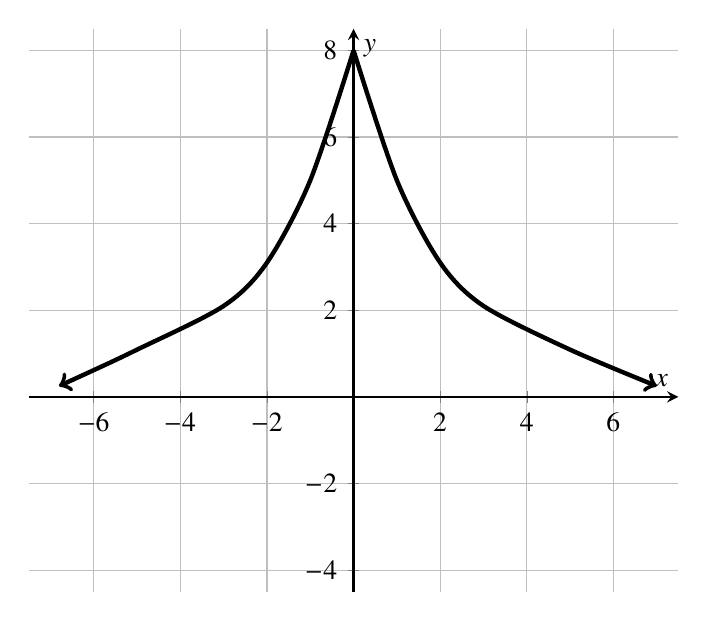
\begin{tikzpicture}
\begin{axis}[x=1cm,y=1cm,scale=0.55,xscale=1, thick, my style, xtick={-6,-4,-2,...,6}, ytick={-4,-2,...,6,8},xmin=-7.5, xmax=7.5, ymin=-4.5, ymax=8.5, mark size=3.0pt, grid = major]
\draw [ultra thick,->] plot [smooth] coordinates { (0,8)  (1,5) (2,3.1) (3,2.1) (5,1.09) (7,0.25)};
\draw [ultra thick,<-] plot [smooth] coordinates { (-6.8,0.25)  (-5,1.09) (-3,2.1) (-2,3.1) (-1,5) (0,8) };
\end{axis}
\end{tikzpicture}
&
%%G' location
\begin{tikzpicture}[scale=0.4]
\draw[->,thick](-10,0)--(10,0);
\draw[->,thick](0,-10)--(0,10);
\node at (10,.4){$x$};
\node at (0.4,10){$y$};
%\node at (-9,3){\large{$g'(x)$}};
\end{tikzpicture}
\end{tabular}
%%%% End FIGURE

\newpage
%%%%Tangent line

\item (12 points) The function $g(x)=x^2(x-1)+4$ is graphed below.

\begin{tikzpicture}[yscale=0.6,xscale=1.8]
  \draw[->] (-2.5, 0) -- (2.5, 0) node[right] {$x$};
  \draw[->] (0, -7) -- (0, 10) node[above] {$g(x)$};
  \draw[<->, domain=-1.9:1.9, smooth, variable=\x, ultra thick] plot ({\x}, {\x*\x*(\x-1)+5});
  \foreach \i in {-2,-1,1,2}{
  	\draw (\i,-.5)--(\i,0.5);
	\node at (\i,-1.3){\i};
	}
%\draw (-.1,25)--(0.1,25);
%\node at (-0.5,25){25};
\end{tikzpicture}
\vspace{0.5in}
	\begin{enumerate}
	\item Sketch and label the \emph{tangent} line to the graph of $g(x)$ when $x=-1.$ \\
	
	\item Write an equation of the tangent line to $g(x)$ when $x=-1.$
	\vfill
	\item Find all $x$-values where the graph of $g(x)$ has a horizontal tangent or explain why none exist.
	\vfill
	\end{enumerate}


\newpage

\item (15 points) Find the derivative of each function below. You do not need to simplify your answer. 
	\begin{enumerate}
	\item $f(x)=2x^{5}+\frac{2}{x^5}+2\sqrt{5}$
	\vfill
	\item $H(\theta)= \theta^{\small{2/3}} \sin(\theta)$
	\vfill
	\item $j(x)=\frac{x}{\pi+\cos(x)}$
	\vfill
	\end{enumerate}
	
\item (6 points) The function $V(T)$ models the volume of a fixed mass of gas with respect to temperature where volume $V$ is measured in milliliters (or $mL$) and temperature $T$ is measured in kelvins (or $K$).
	\begin{enumerate}
	\item Interpret in the context of the problem the meaning of $V(100)=60.$ Include units.
	\vfill
	\item Interpret in the context of the problem the meaning of $V'(100)=0.4.$ Include units.
	\vfill
	\item Using the facts that $V(100)=60$ and $V'(100)=0.4,$ estimate $V(110).$ Include units.
	\vfill
	\end{enumerate}
\newpage
\item (17 points) A spring is hanging from the ceiling with a mass attached to it. The mass is oscillating vertically with simple harmonic motion. The function $h(t)= 6-\cos(t)$ models the height of the spring above the floor starting at time $t=0$ where $h$ is measured in feet and $t$ is measured in seconds.
\emph{For all problems below, include appropriate units.}

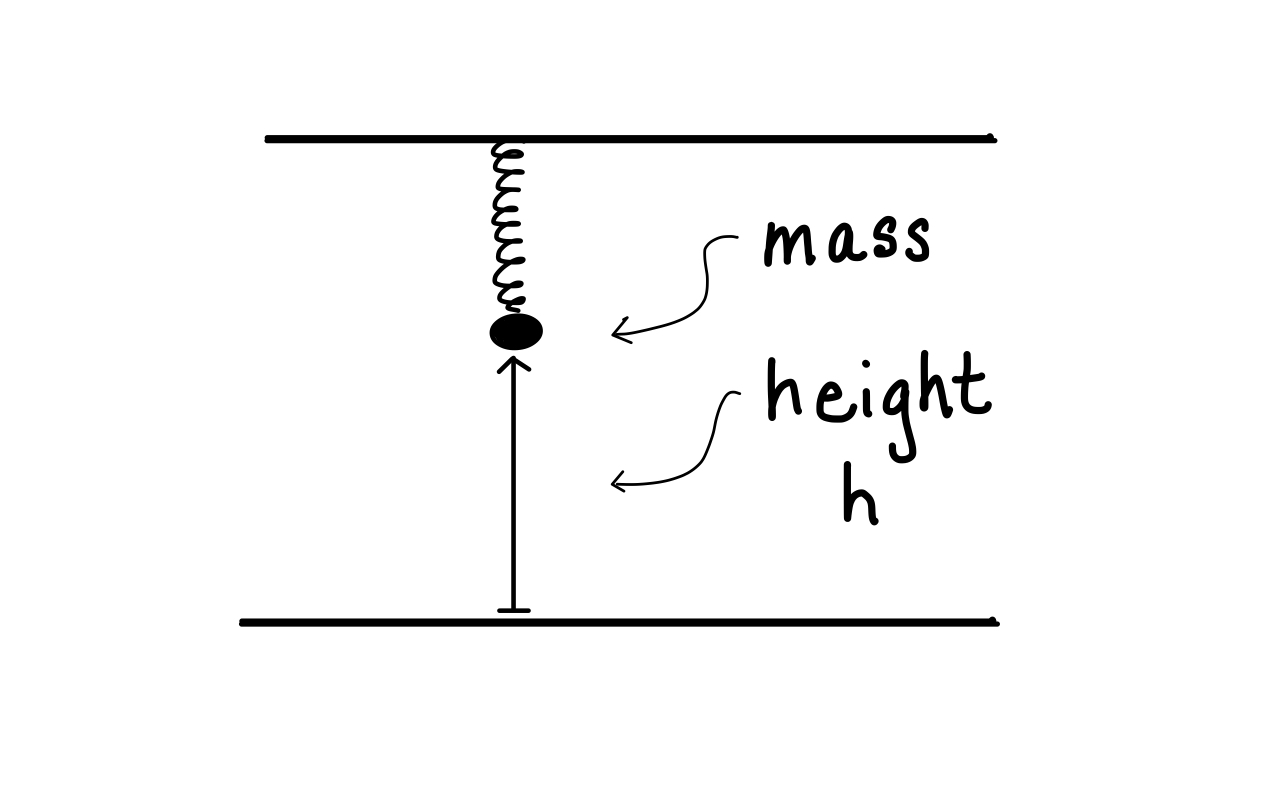
\includegraphics[scale=0.2]{spring.jpeg}

\vspace*{-.5in}

	\begin{enumerate}
	\item Find the average velocity of the mass in the time interval $[0, \pi]$ seconds.
	\vfill
	\item Find the equations for the velocity and acceleration of the mass.\\
	\vfill
	\item Find the instantaneous velocity of the mass at $\pi/4$ seconds.\\
	\vfill
	\item At $t=\pi/4,$ is the mass going up or going down? Justify your answer.\\
	\vfill
%	\item At $t=\pi/4,$ is the mass speeding up or slowing down?\\
%	\vfill
	\item Determine all times $t>0$ at which the mass changes direction?
	\vfill
	\end{enumerate}
\end{enumerate}
\newpage
\textbf{Extra Credit:} (5 points) Use the Intermediate Value Theorem to demonstrate that the function $f(x)=x^3-3x-19$ has a root (or zero) in the interval $[1,5].$  A complete answer requires some calculations \emph{and} complete sentences justifying your conclusion.
\vspace{2.5in}
\end{document}

%%%%ENDDOCUMENT


